\section*{Experiment 2}

For a single value of the inverting input voltage, we then swept the
non-inverting input around the inverting one while measuring \Vout. We then fit
a straight line to the steep portion of the curve in order to determine the
differential-mode voltage (\Adm) gain of the circuit. The experimental results,
along with the differential mode gain fit to the curve is shown in Figure
\ref{fig:exp2p1}.

From the experimental data, we found $A_{dm} \approx 110$
\begin{figure}[H]
\centering
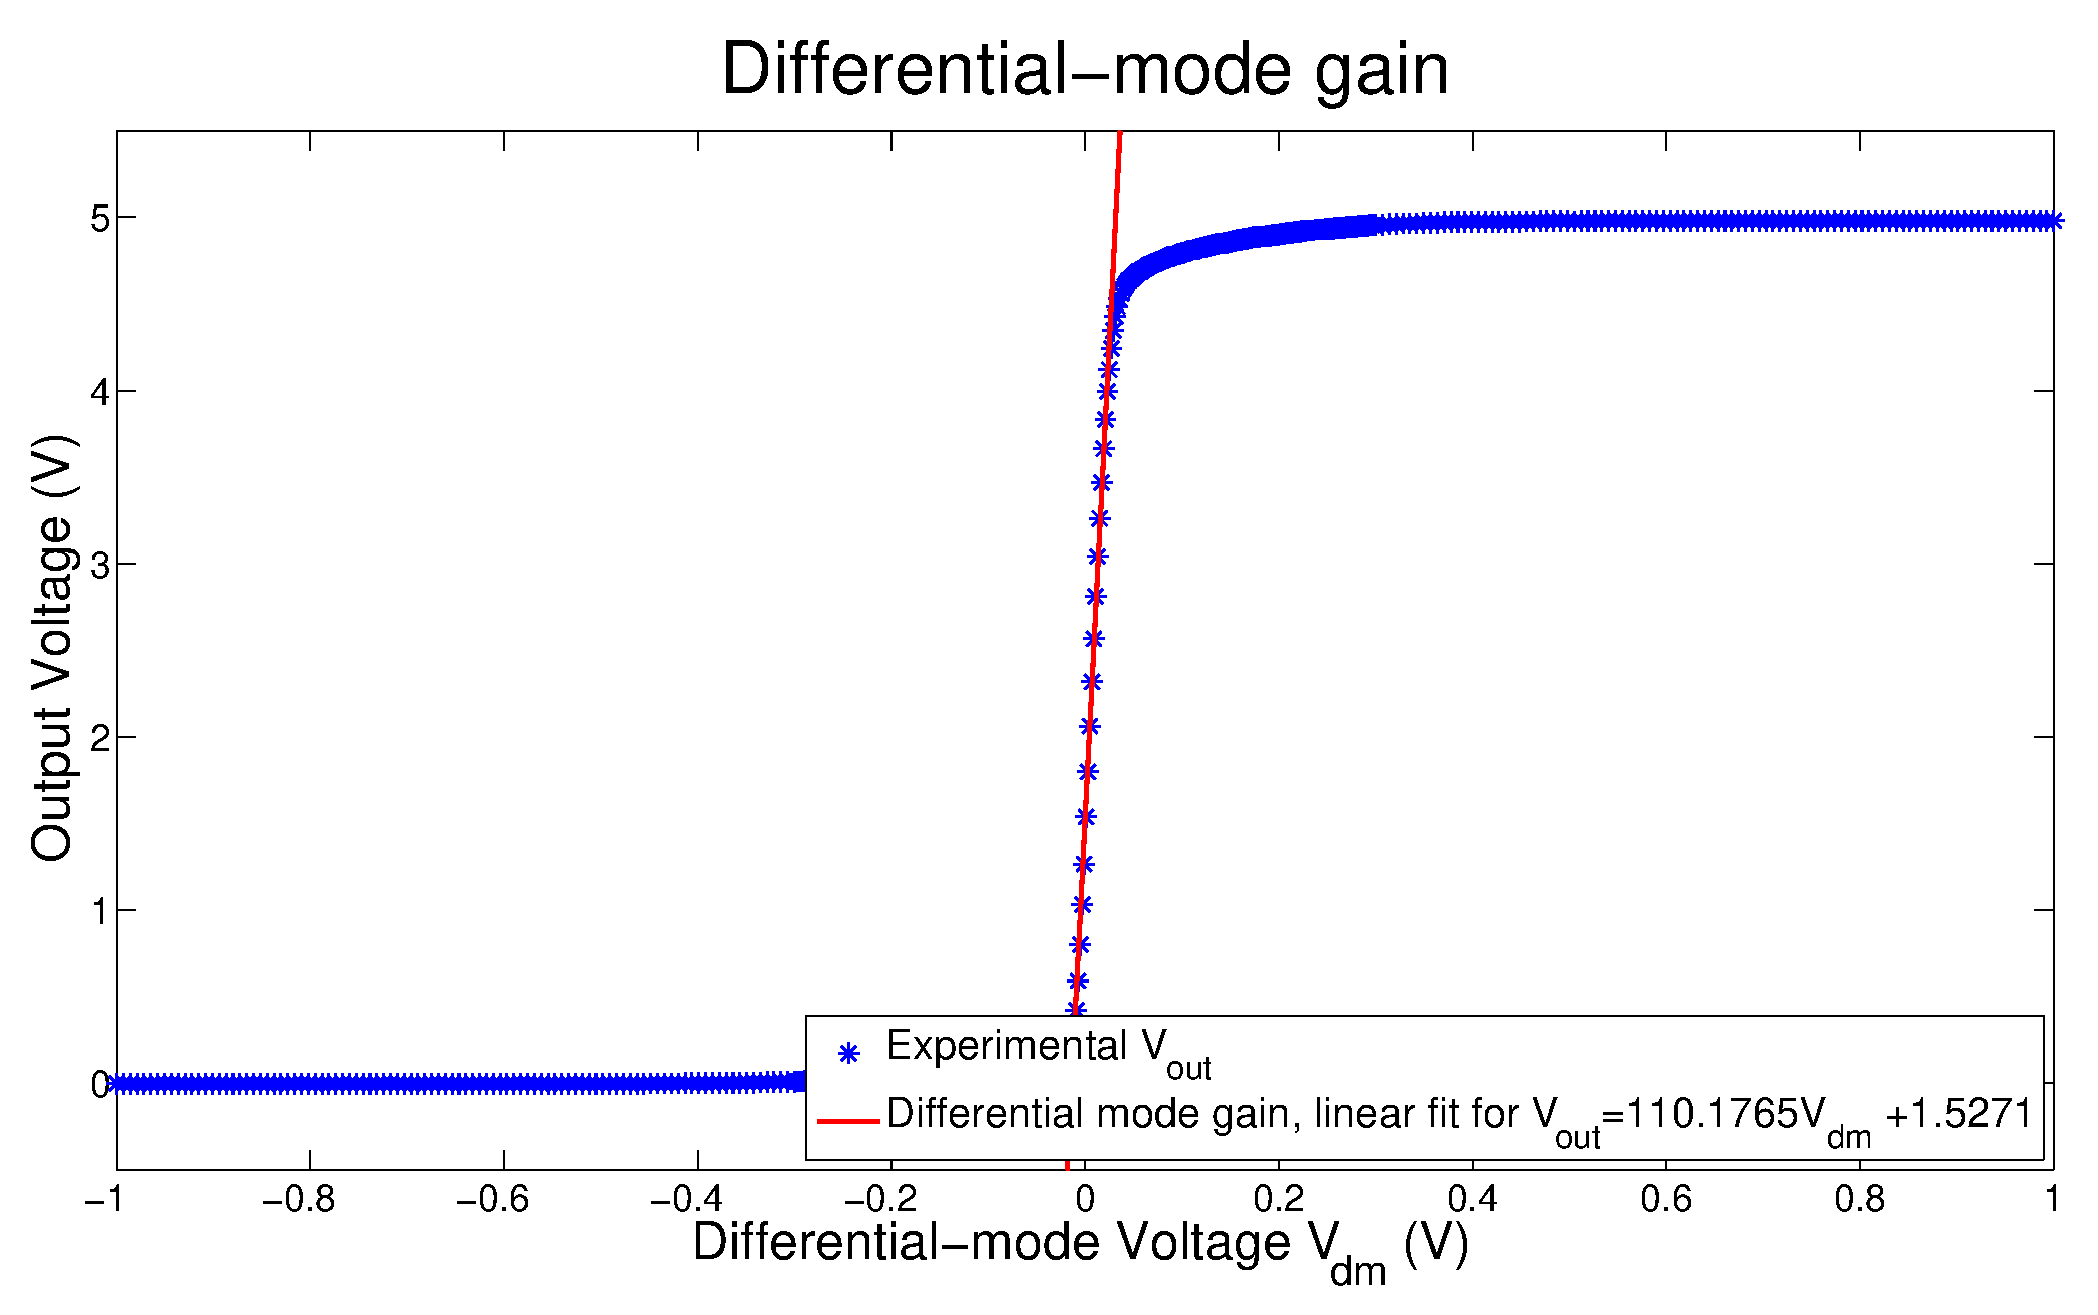
\includegraphics[width=\linewidth]{../Figures/Exp2P1.eps}
\caption{}
\label{fig:exp2p1}
\end{figure}

Next, we set the differential-mode input voltage to zero and measured the
current flowing into the output of the amplifier as we swept \Vout from one
rail to the other. We fit a straight line to the shallow part of this output
current–voltage characteristic in order to determine the incremental output
resistance of the circuit. The voltage transfer characteristic in this region
can be seen below in Figure \ref{fig:exp2p2}.
From the linear fit, we extracted an incremental output resistance of $489.6k\Omega$.

\begin{figure}[H]
\centering
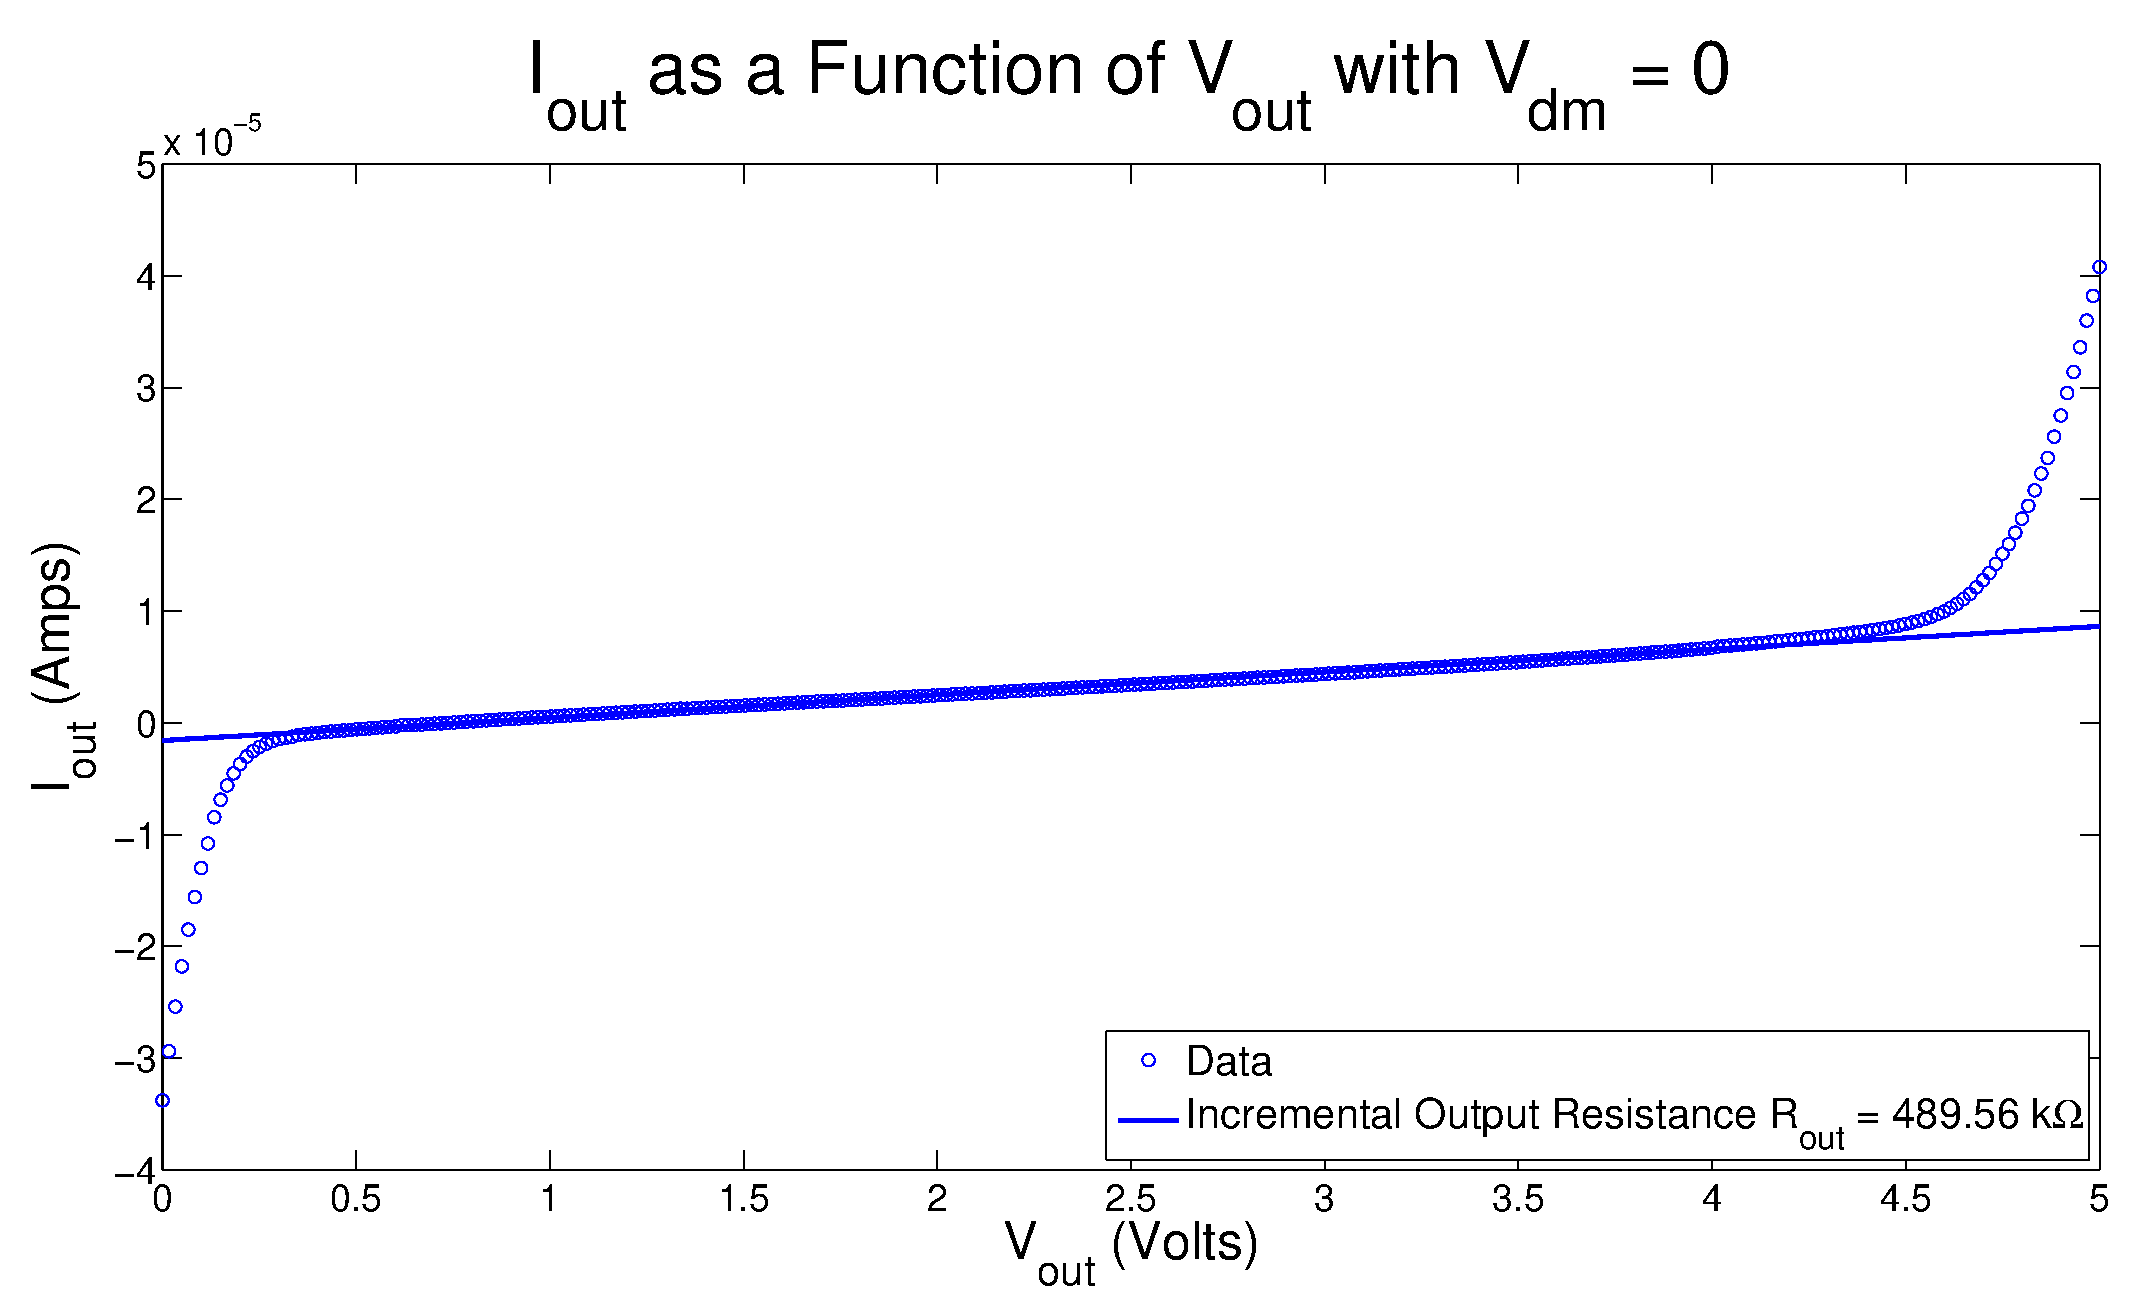
\includegraphics[width=\linewidth]{../Figures/Exp2P2.eps}
\caption{}
\label{fig:exp2p2}
\end{figure}

Next, we fixed the output voltage at $2.5V$ and measured the current flowing
out of the amplifier as we swept \Vdm around zero. We then fit a straight line
to the curve around where $V_{dm} = 0$ in order to extract the incremental
transconductance gain of the circuit.  This voltage transfer characteristic 
can be seen in Figure \ref{fig:exp2p3}.
From the linear fit, we extracted an incremental transconductance gain of $2.3687 \times 10^{-4} \Omega^{-1}$

In this experiment, we found the limiting values of $I_{out}$ to be $+ 66.69 \mu A$, and $-70.01 \mu A$, fairly symmetric on both rails. 

We then calculated the differential-mode gain of the circuit by computing
the product of \Gm and \Ro.
$$A_{dm`} =  2.3687 \times 10^{-4} \Omega^{-1} \cdot 489.6k\Omega = 115.477$$
This theoretical differential-mode gain is slightly higher than our extracted
value, of $110$. This represents a relative percent error of roughly $4.9\%$.

In comparison to our previous lab's VTC and \Adm value, this circuit is a much better amplifier. It not only can achieve a larger range of output voltages, with a rail-to-rail swing, but the differential-mode-gain is almost twice that of Lab 8's amplifier. In Lab 8, we found $A_{dm} = 62.4146$. Thus this amplifier is far more reactive to small changes in voltage and would be more useful in the real world!


\begin{figure}[H]
\centering
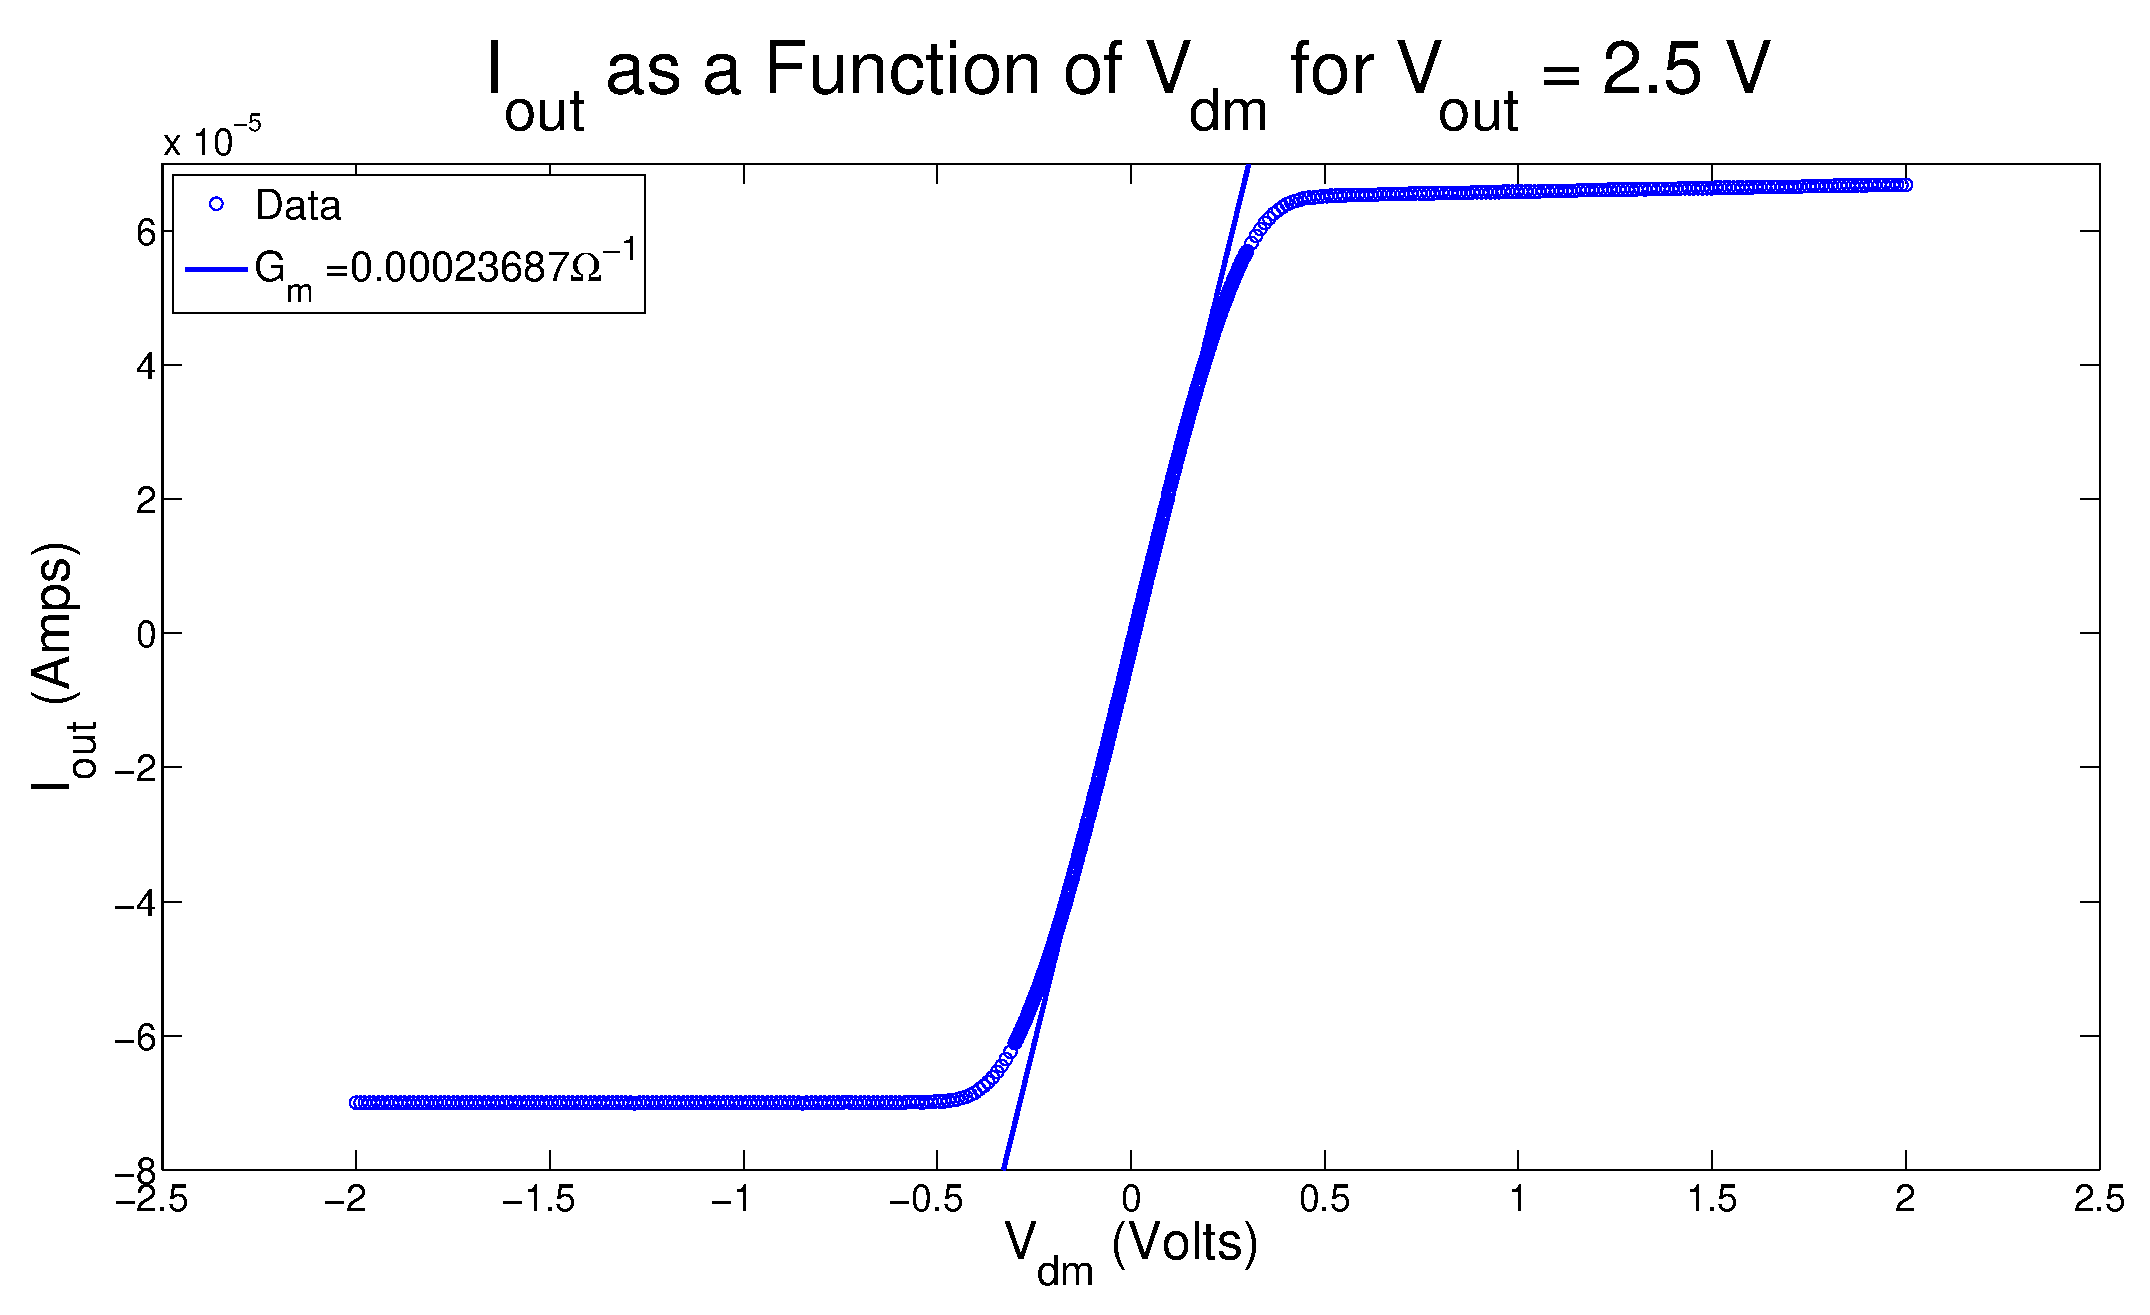
\includegraphics[width=\linewidth]{../Figures/Exp2P3.eps}
\caption{}
\label{fig:exp2p3}
\end{figure}